\documentclass[twoside,letterpaper,twocolumn]{article}

%%%%%%%%%%%%%%%%%%%%%%%%%%%%%%%%%%%%%%%%%%%%%%%%%%%%%%%%%%%%%%%%%%%%%%
% Package with format specifications for the 9th CISBGf
\usepackage{cisbgf}


%%%%%%%%%%%%%%%%%%%%%%%%%%%%%%%%%%%%%%%%%%%%%%%%%%%%%%%%%%%%%%%%%%%%%%
% MANDATORY PARAMETERS

% Setting the title
\title{Data Management of BRASIS -
BRAzilian Integrated Seismological Network}

% Setting the authors
\author{Bruno Colla\c{c}o, Jackson Calhau, Marlon Pirchiner, Sergio Jr. S. Fachin, Marcelo
Assump\c{c}\~{a}o, IAG/IEE-USP Seismological Center, Brazil}

% Setting the headings
\headauthor{Pirchiner, Collaço, Calhau et al.}
\headtitle{Seismological Data Management}

%%%%%%%%%%%%%%%%%%%%%%%%%%%%%%%%%%%%%%%%%%%%%%%%%%%%%%%%%%%%%%%%%%%%%%
%%%%%%%%%%%%%%%%%%%%%%%%%%%%%%%%%%%%%%%%%%%%%%%%%%%%%%%%%%%%%%%%%%%%%%
\begin{document}

\maketitle

\begin{abstract}

Historically, the brazilian seismology never had a strategic and solidified vision about how its data should be acquired, evaluated, stored and made available. Without good data management systems, good quality data acquired can be lost foverer, more time can be spent in querying and preparing datasets for analyses and also local and international colaboration will probably be reduced, in other words: a lot of data will never become scientific knowledge. With the emergence of BRASIS (Pirchiner et al, 2011) besides the significantly increase in the amount of data being acquired at the IAG/IEE-USP Seismological Center (SC), a chance was opened to implement a suitable data management plan to cover this shortcoming. This work describes the efforts of the SC to set up a seismology data management system which addresses data life cycle as it has been discussed by the international community.

\end{abstract}

\section{Introduction}

Digital seismology started at SC at the early 1990's. Several temporary seismological experiments have been carried out in many areas of the Brazilian shield. For many years, a large amount of data obtained was stored on various media and in different formats, making the use of this data by other institutions very complicated. In 2008, those data issues emerges unsustainable: a lot of data stored in old tapes were not readable anymore, hard disks crashed and the mistaken decision to store only earthquake data (to save disk space) made some kind of studies (eg. ambient noise tomography) impossible. It was clear that something needed to be done to preserve the data still useful. 

After some IRIS (Incorporated Research Institutes for Seismology) workshops, the SC started to assemble SEED (Standard for the Exchange of Earthquake Data) volumes to be stored at IRIS. Furthermore, much time was spent translating field sheets into metadata archives which contain the site and equipment information. This hard work brought experience to SC on how to care of seismological data. At the end of 2009, all data of 15 years of deployment was stored and made available at the IRIS Data Management Center unde ther BL network code, accessible for everyone by using a wide range of tools.


\section{The BRASIS Project}

BRASIS is the most important project in which the SC is envolved since 2009, when the brazilian oil company PETROBRAS approved its funding. BRASIS is part of a bigger project carried out by more three other institutions that are deploying the brazilian permanent seismological network, something that the country never had before (earlier projects were local or regional temporary experiments). The locations of the stations which were already deployed can be seen in Figure 1. 

For the acquisition, real-time processing and data dissemination, the SC has chosen the german SeisComP3 as the main software running in its datacenter for many reasons: "no" cost; open source; use of GNU/Linux operating system; possibility of local maintenance; participation in future developments; and framework platform to easily develop local tools.

\begin{figure}[h!]
\centering
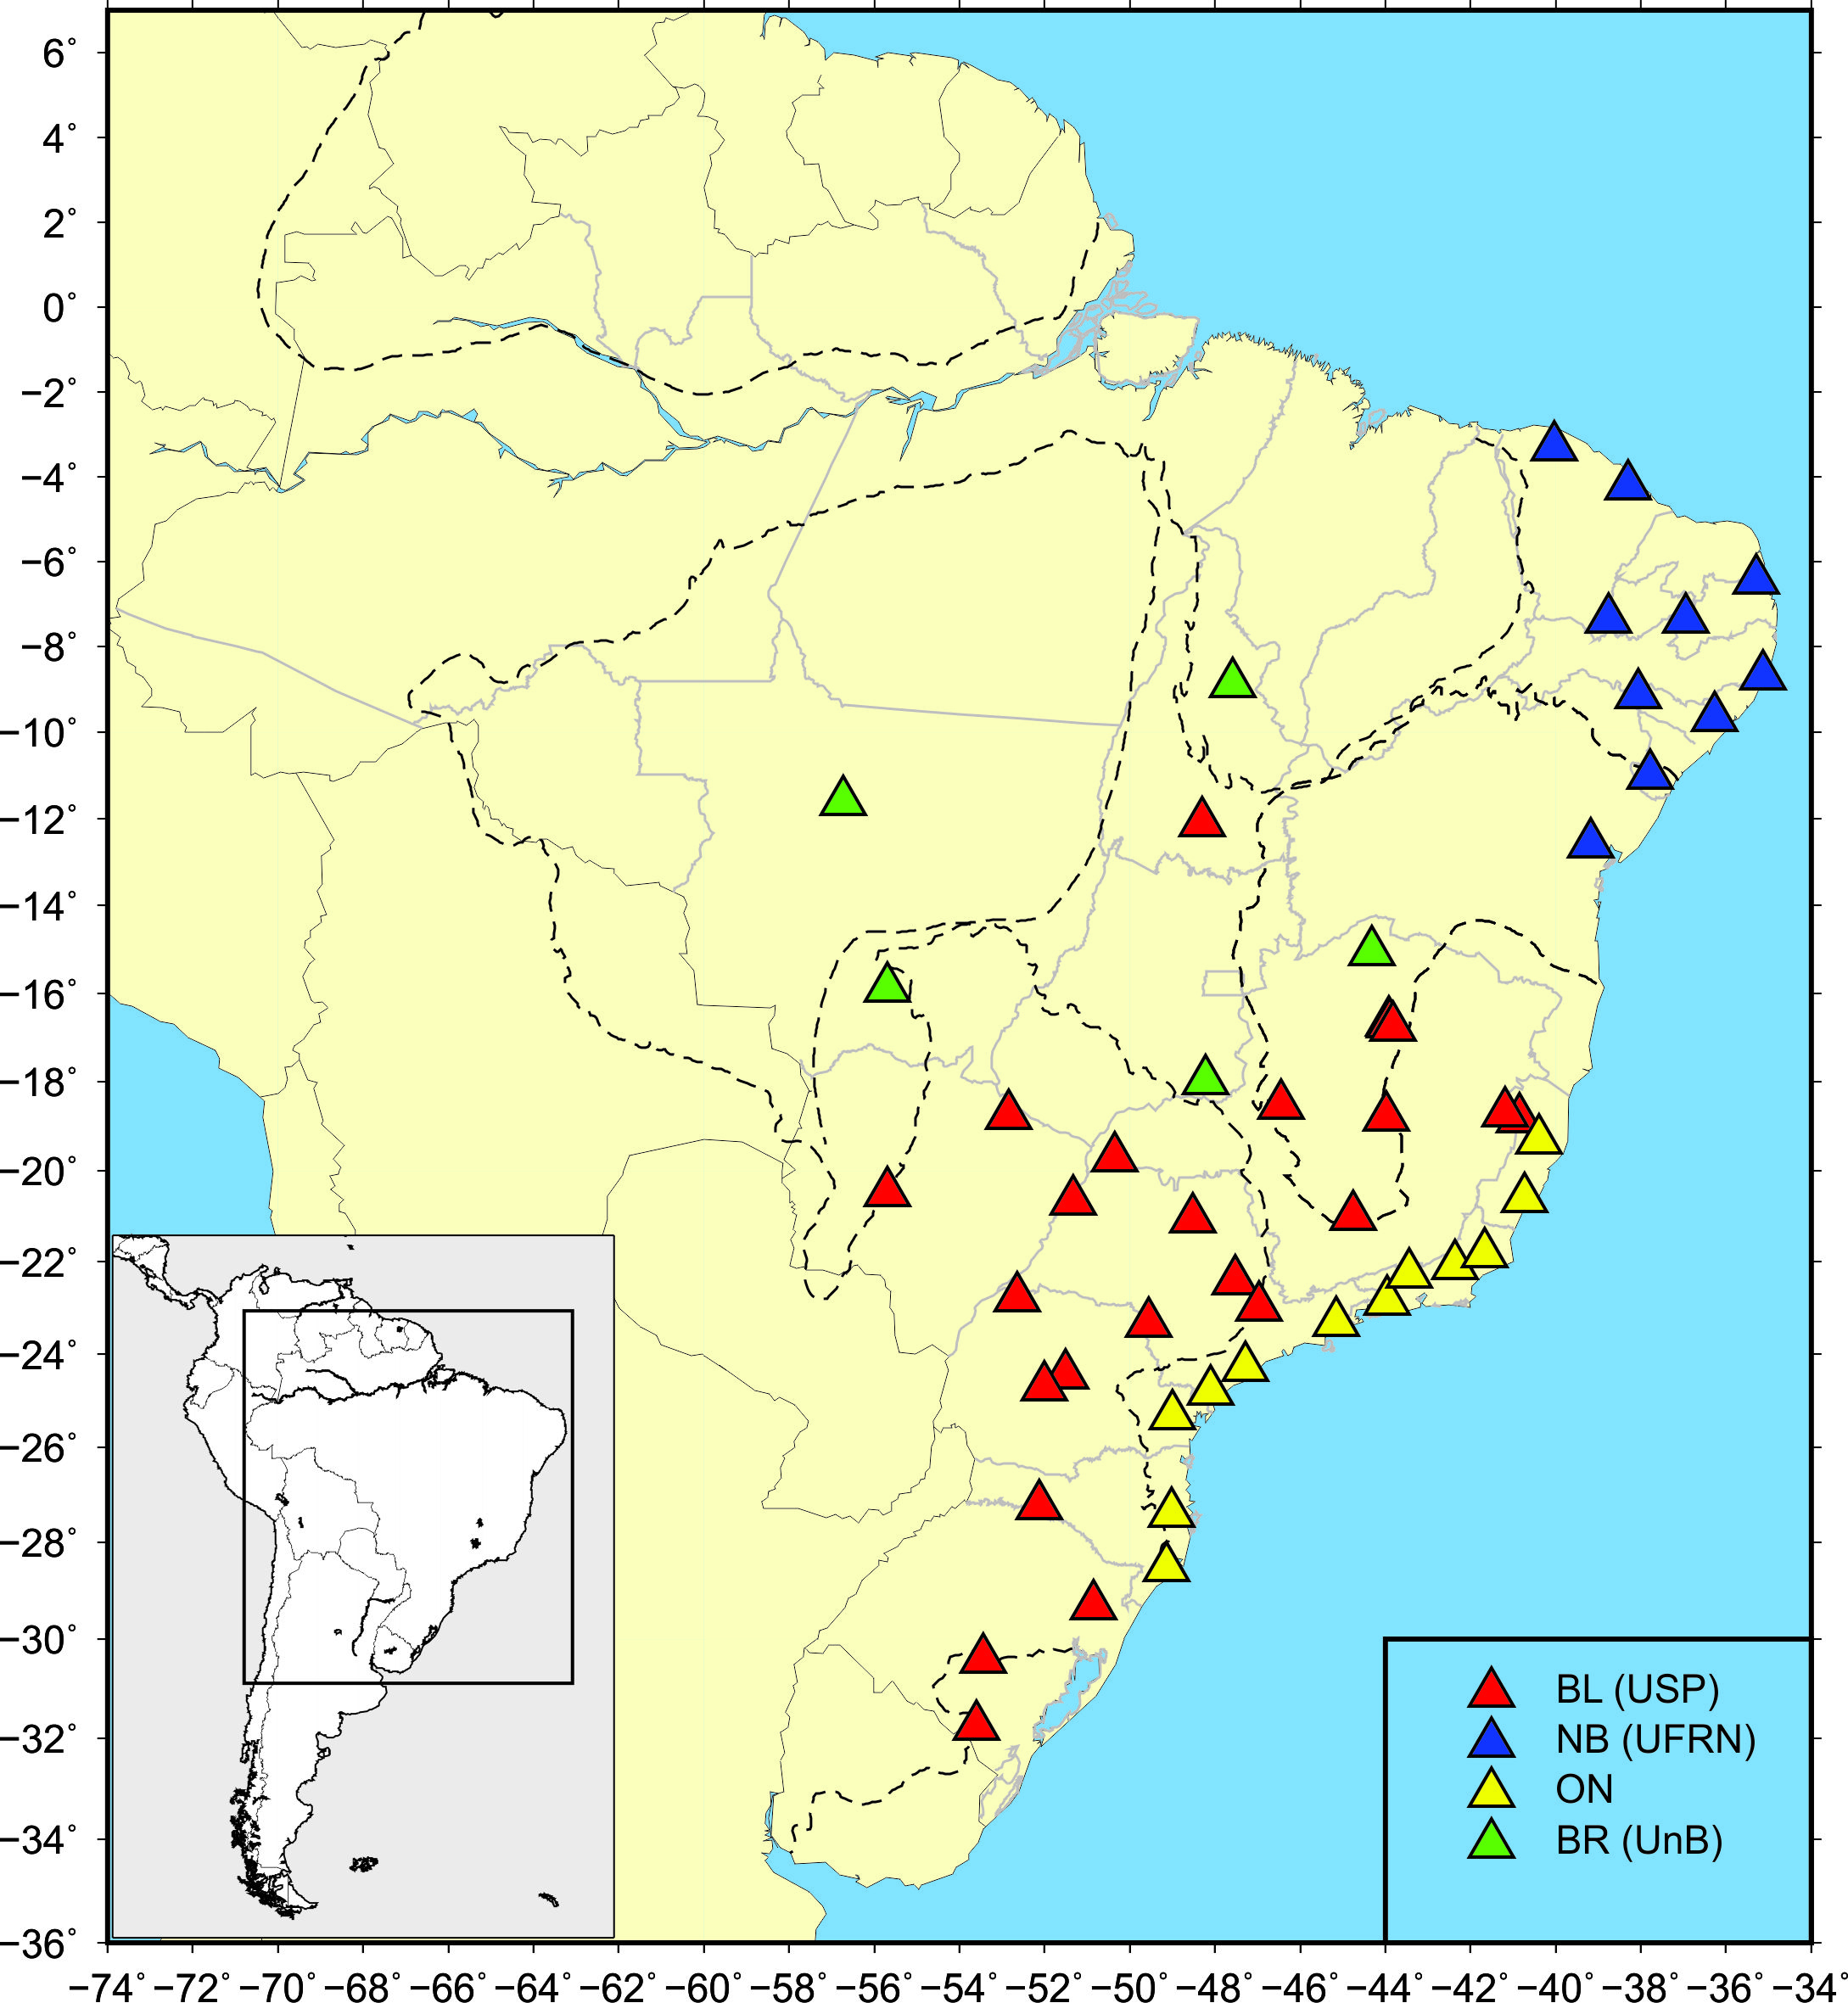
\includegraphics[width=7.8cm]{images/rsb.jpg}
\caption[Figure 1]{Actual deployment status of the brazilian seismological network: red triangles are stations from BRASIS. Blue triangles are stations deployed by the Rio Grande do Norte University (UFRN). The yellow triangles along the coast are stations from the National Observatory (ON). The University od Brasilia (UnB) deployed the stations represented by the green triangles. }
\end{figure}

Since May 2011 to April 2013, the BRASIS network has detected about 600 events with magnitudes between 4 and 7.2, most of them at the Andean region. 75\% of the events with magnitudes 5+ were located with less than 15km error when compared with the NEIC catalog. The automated magnitudes were also computed with an error of  $ \pm $ 0.35. Regional brazilian earthquakes were not located automatically because a magnitude 4+ did not occur yet. However, smaller events are being detected manually. The SC also mantains a catalog of the earthquakes that occur in Brazil. This catalog is open and accessable through the SC website at \textit{www.sismo.iag.usp.br/portal}, where one can also find information about the stations and retrieve its data. Furthermore,  a \textit {GeoServer} instance is running at the SC's datacenter, offering both station and earthquake catalog in raster formats, at \textit{www.sismo.iag.usp.br/geoserver}.

\section{Data Life Cycle at the Seismological Center}

Beyond the characteristics of the seismological data acquisition, Figure 2 shows that there are basically two ways to add data to the system: in real-time or with archives brought by a station technician. The data management plan at the SC intended to handle internally all the waveform acquired with the same procedures to facilitate its access and reuse.

\begin{figure}[h!]
\centering
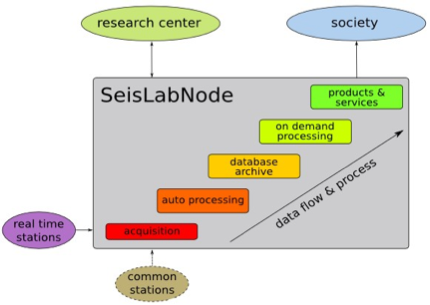
\includegraphics[width=7cm]{images/dataFlow.png}
\caption[Figure 2]{Data processing model at the Seismological Center. This diagram shows which skills a data center need to have to properly handle its data. It shows data exchange, and internal data flow and processes.}
\end{figure}

The steps of a waveform life cycle (Figure 3) can be separated in three different phases: acquisition, curation and preservation, as described below:

\textbf{a) \textit{Acquisition}}
\begin{itemize}
\item \textit{Deployment:} from site selection to sensor installation procedures, all the cares of generation of good quality data;
\item\textit{Station Metadata:} made with factory's instrument data sheet in a proprietary format used to configure the instrument and to remove its response at the waveform processing step;
\end{itemize}

\textbf{b) \textit{Curation}}
\begin{itemize}
\item \textit{Ingestion:} waveform data arrives at the datacenter in a propetary format. Then, it is extracted wth acquisition logs and converted to an open format (SEED). The station metadata is added at this step, to describe it in the same open standard (dataless SEED format;
\item \textit{Quality Control:} acquisition logs like GPS lock timing, data gaps and noise evaluation (power spectral density plots) are made to garantee the quality of the acquired data;
\item \textit{Data Dissemination and Access:} both miniSEED and datalessSEED archives are served for free access in real-time or on demand by the SC's SEEDLink and ArcLink Serves at \textit{seisrequest.iag.usp.br} (port 18000 for SEEDLink and 18001 for ArcLink);
\item \textit{Real Time Processing:} the SeisComP3 system processes all the data that is being acquired in real-time. When an event is detected, the system runs its automated locators and magnitude calculators. The product, an event in the QuakeML format is stored at the database with its associated objects: picks, phase arrivals, origins, agency code, etc;
\item \textit{Revision:} later, an analyst review each event detection to refine its location;
\end{itemize}

\textbf{c) \textit{Preservation}}
\begin{itemize}
\item \textit{Hardware:} all the systems at the SC's datacenter run on hardware prepared for redundancy;
\item\textit{Storage:} all the SC's data products are stored in a RAID 5 dedicated storage;
\item\textit{Long Term:} all the SC's data products are open and are also being stored and the IRIS DMC servers;
\end{itemize}

\begin{figure}[ht!]
\centering
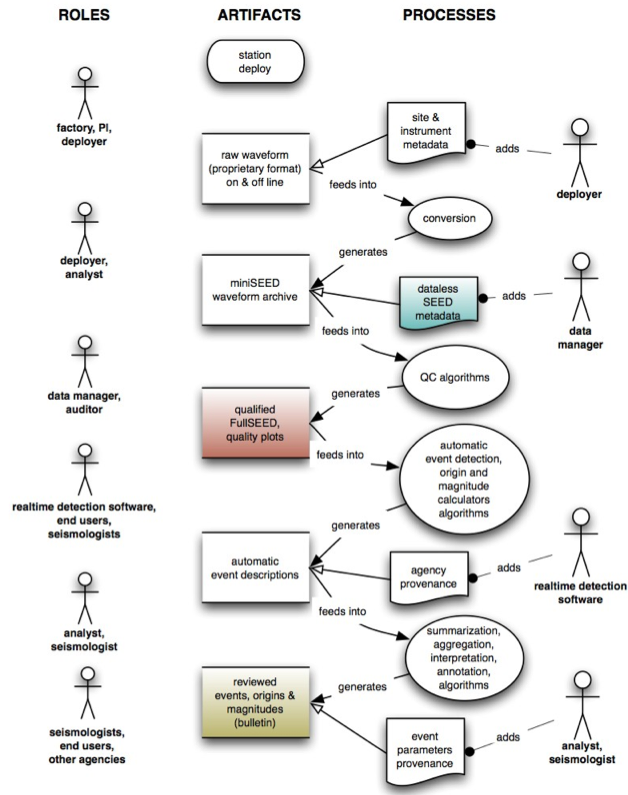
\includegraphics[height=10cm]{images/dataSteps.png}
\caption[Figure 3]{A simplified waveform life cycle. The colored artifacts are consider the most important by the major part of the community}
\end{figure}

\section{Open Questions, Next Steps}

Seismologists together with students when are working on their researches uses and also generates a lot of seismological objects like picks, amplitude readings, earth models, filtered seismograms, dispersion curves and tomographic maps among others. When the work in cooperation is needed in a distributed way or not, the problem to describe who did what is still open and the best solution is not easy to find. 

Figure 4 illustrates a schematic representation of the data infrastructure installed at the SC's datacenter. However, some questions were not answered yet.

Which is the best way to care about all of these seismological \textbf {related and distributed data}? How to manage all these processes and how to catch the \textbf {provenance} of these objects correctly? \textbf {Semantic} technology could be useful for this task? If so, how to implement semantic issues on this case study? In this context, does it make any sense to move towards a \textbf {virtual observatory} concept?

\begin{figure}[ht!]
\centering
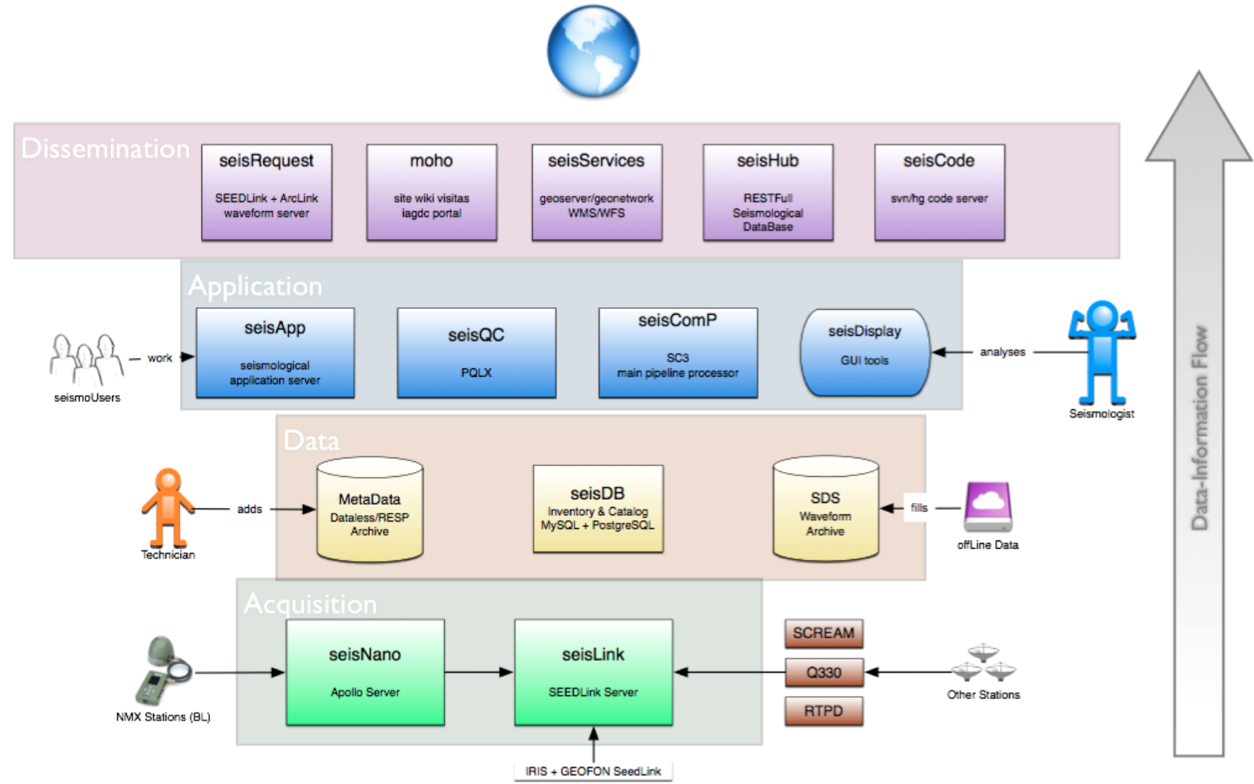
\includegraphics[width=8cm]{images/datacenter.png}
\caption[Figure 4]{Schematic infrasctructure representation with basically four distinct layers of the data flow, described from bottom to top. First layer represents data acquisition by two mainly services. The second layer is where seismological data (waveforms and associated data) is stored. Seismological applications runs at the third layer, where students and seismologist can interact with the data. The fourth and last layer is about data dissemination, where the SC's products are offered to the community.}
\end{figure}

\section{Comments and Conclusions}

The culture of do not plan to make a properly curation of acquired data and preserve it to future reuse, contributes to make the management task a little harder. 

In Brazil, funding agencies do not ask for data management plans, leaving the responsability to each researcher.The cost of maintaining and preserving data is high and is often not taken into account when projects are signed. Frequently there is no budget nor people to do this job.

The BRASIS project was the very responsible for changing the SC's efforts to data management issues. Despite the difficulties, the SC is doing the best it can to match and comply the best practices in seismological data management as adopted by the international community.

To manage data correctly is not an easy task. Management plans made earlier would greatly help to estimate what is needed for a proper treatment and preservation of the acquired data and also the cost involved. A lot of problems emerges from the fact of have no plan.

To broaden the discussion of data management plans among other institutions and researches is essential to join efforts and reduce costs. The concept of a Virtual Observatory emerging from this whole data management, providing well known and new services could be a horizon to follow.  


\section{References}

Barsh, R. (2009) Web-based technology for storage and pro- cessing of multi-component data in seismology. First steps towards a new design, PhD thesis, Ludwig Maximilians Universitat Munchen, Munich, Germany, 126 pp.

Percivall, G. (2010). The application of open standards to en- hance the interoperability of geoscience information, In- ternational Journal of Digital Earth, 3 (S1), 14-30.

Pirchiner, M ; Collaço, B. B. ; Calhau, J. ; Assumpção, M. S. ; Dourado, J. C. . BRAzilian Seismographic Integrated Systems (BRASIS): infrastructure and data management. Annals of Geophysics, v. 54, p. 17-22, 2011.

Schorlemmer, D., A. Wyss, S. Maraini, S. Wiemer and M. Baer (2004). QuakeML - an XML schema for seismology, ORFEUS Newsletter, 6 (2); http://www.orfeus-eu.org/Organiza- tion/Newsletter/vol6no2/quakeml.shtml (last accessed 7 March 2011).

SEED Manual (2010). SEED Reference Manual, SEED Format Version 2.4, May 2010, IRIS, 212 pp.; 

SeisComP3.org (2011). SeisComP 3 documentation; www.seiscomp3.org/wiki/doc (last accessed 20 April 2013).



\section{Acknowledgments}

We would like to thank PETROBRAS for funding the BRASIS Project and also the SC's staff, specially Marcelo Assumpção for the support and trust.

\end{document}